% !TEX root = ../../../Lazcorreta.Tesis.tex
Los datos recogidos por la entidad que quiere hacer el proceso completo de \KDD pueden ser de diferente índole, incluyendo datos personales que no deberían ser accesibles por todos los investigadores involucrados en el proceso de \KDD. La primera fase del proceso es la selección de atributos que serán realmente analizados entre los disponibles por la entidad propietaria de los datos. Los investigadores tendrán a su disposición lo que en la figura~\ref{fig:fasesProcesoKDDFayyad} se denomina \texttt{Target Data}, que realmente es una consulta realizada a la \db completa, \texttt{Data}. Aquí aparece por primera vez el caracter recursivo de este proceso: si los investigadores determinan que necesitan datos que ni siquiera están recogidos en la \db global podrían solicitar a la entidad la obtención de dichos datos, afectando al punto de origen del proceso.

\begin{wrapfigure}{o}{0.45\textwidth}
  \centering
  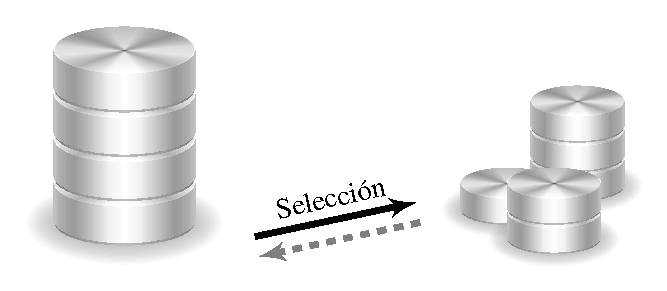
\includegraphics[width=.45\textwidth]{Seleccion.pdf}
	\caption{Selección de datos}
	\label{fig:SeleccionDeDatos}
\end{wrapfigure}
Esta selección es fundamental para el proceso global de \KDD, si los resultados de la evaluación final no son satisfactorios pueden provocar que se opte por una selección diferente de los registros y campos a incorporar en el \texttt{Target Data}. Cualquier decisión errónea en esta fase puede derivar en análisis que no conduzcan al descubrimiento real de conocimiento útil y previamente desconocido sobre la población en estudio.

Si la \db en estudio pertenece a una empresa (pública o privada) son los responsables de la misma quienes han de decidir, aconsejados por los investigadores que llevarán a cabo el proceso de \KDD y por las leyes vigentes en el país en que se realiza el estudio, qué datos y registros pasan a formar parte del \texttt{Target Data}, recurriendo a la codificación de los datos que sean necesarios para el análisis pero no deban aportar información sensible.

La selección en sí, unida a la experiencia de los investigadores encargados del proceso de \KDD, determinará si se han de recabar en \texttt{Data} atributos y datos necesarios para el objetivo perseguido. Todas las fases del proceso son recurrentes y pueden generar parte del conocimiento buscado en el sentido de obligar a retroceder en el proceso para mejorar la calidad del conocimiento final adquirido. 

En el caso de la \WUM existen datos recogidos en el servidor al atender a demandas internas de sus usuarios, con información confidencial sobre los usuarios o sobre la estructura o contenido del sitio web. Este tipo de información no debería ser accedida por quienes analizan el uso del sitio web por lo que debería ser filtrada durante esta primera fase. Si fuera necesario se podrían codificar las propias IPs de los usuarios del sitio u otros datos que pueden revelar información personal para cumplir con las normativas sobre privacidad de datos del país en que se está llevando a cabo la investigación\citep{LamFrankowskiRiedl-DoYouTrustYourRecommendations-2006,RozenbergGudes-ARMInVerticallyPartitionedDBs-2006}.
